\documentclass[a4paper]{article}
\usepackage{graphicx}
\usepackage{mathtools}
\usepackage{amsmath}
\usepackage{amsthm}
\usepackage{amssymb}
\usepackage[a4paper,top=1cm,bottom=2cm,left=3cm,right=3cm,marginparwidth=1cm]{geometry}
\graphicspath{ {./images/} }
\renewcommand{\baselinestretch}{1.3}

\title{ IKV1 homework - Hypotheses Testing on ETRA Challenge dataset }
\author{Martin Picek }
\date{December 2021}

\newcommand{\irow}[1]{% inline row vector
  \begin{smallmatrix}(#1)\end{smallmatrix}%
}

\begin{document}

\maketitle

\section{Introduction}

In ETRA Challenge, 8 subjects were tested on various tasks including visual fixation, visual search, and visual exploration. Multiple stimuli were presented, for example,
natural images, blank scenes, or a pictures scanned from Where's Waldo book. Based on the data, we came up with two hypotheses:
\begin{enumerate}
    \item Pupil size is the same on blank and natural stimuli (during free viewing task).
    \item Maximal pupil size is different when Waldo is found (during free viewing task).
\end{enumerate}

\section{Data format}

The dataset is divided into two parts. The file \texttt{DataSummary.csv} where each trial has one row with clicks on the screen recorded. Then there is the \texttt{data} folder with a subfolder
for each subject. For each trial of a subject, there is a file in the subject's subfolder.

\section{Hypothesis 1: Pupil size is different on blank and natural stimuli (during the free viewing task).}

For this experiment, we collected data of blank and natural stimuli separately (during the free viewing task). For each subject, we obtained the data from trials,
concatenated the corresponding data with regard to stimulus and therefore obtained two data tables - one for natural stimulus, and one for blank stimulus.

Then we performed a statistical test testing whether the means of the two distributions are the same. We obtained a p-value for each subject.

\subsection{What statistical test to use?}

There are many statistical tests that we can choose from. One very widely used is called the T-Test.
This test assumes that the two distributions follow the normal distribution, have unknown standard deviations
and means $\mu_1$ and $\mu_2$. Then the $H_0$ states that $\mu_1 = \mu_2$, alternative $H_1$ states that $\mu_1 \neq \mu_2$.
\\
\\
The p-values obtained are the following: 
\begin{itemize}
    \item Left pupil: $\irow{0&0.1071&0&0&0&0&0&0&}$
    \item Right pupil: $\irow{0&0&0&0&0&0&0&0&}$
\end{itemize}


What we found out is that if the significance level is 2 percent, 7 out of 8 tests rejected the null hypothesis (regarding the left pupil). That means that 7 out of 8
tests returned that the means are different (for the left pupil). On the other hand, p-values for the right pupils were all zeros - meaning all hypotheses are rejected.
\\
\\
However, this test assumes one important property - the distributions follow the normal distribution. But what if they do not?
Here is a plot of left pupil size on blank stimuli of subject 009. Although no similarity test to normal distribution was performed,
it is obvious that the distribution does not resemble the Gaussian curve.

\begin{gather*}
    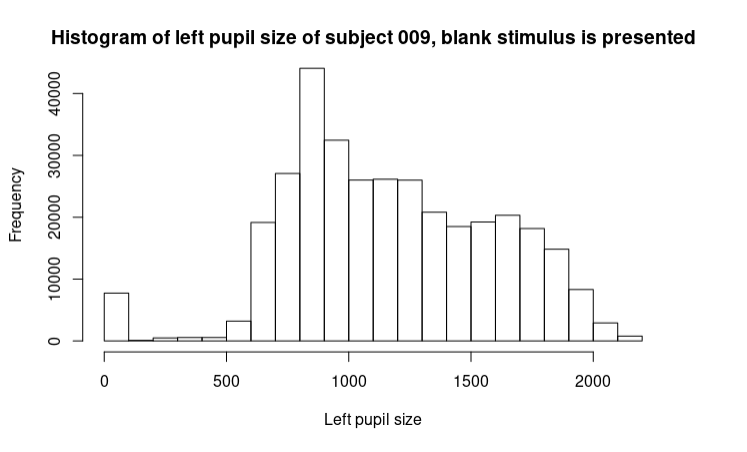
\includegraphics[scale=0.5]{hist1.png}
\end{gather*}

On the other hand, the only test that has p-value larger than the significance level is very similar to the normal distribution.
This is maybe the reason why this is the test with the higher p-value.

\begin{gather*}
    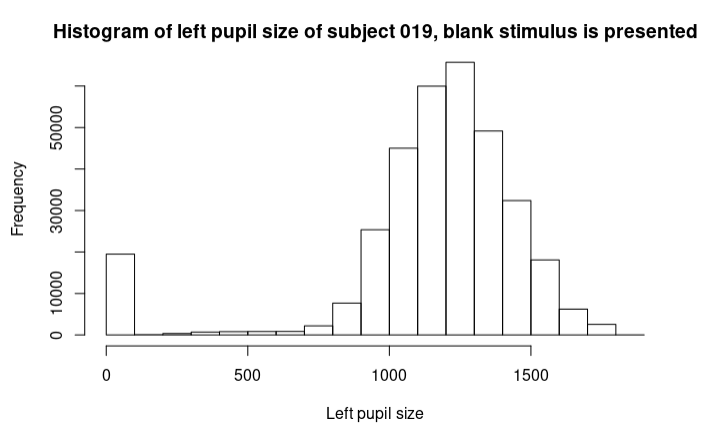
\includegraphics[scale=0.5]{hist2.png}
\end{gather*}
\\
\\

Owing to this observation, we performed the Wilcox rank-sum test. This test is a non-parametric analogy of the T-Test.
While T-Test assumes that the distributions are normal, Wilcox rank-sum test doesn't assume any specific distribution.
It just tests the equality of means.

Let us see the resulting p-values obtained by Wilcox rank-sum test:
\begin{itemize}
    \item Left pupil: $\irow{0&0&0&0&0&0&0&0&}$
    \item Right pupil: $\irow{0&0.3983&0&0&0&0&0&0&}$
\end{itemize}

Now we can see, that the test did not reject the $H_0$ hypotheses for the third subject.

\subsection{Discussion of results}

We discovered that the size of pupils differs between natural and blank stimuli. We came up with the following explanations:

\begin{enumerate}
    \item \textbf{The images are different and therefore evoke different sizes of the pupil.} This might be explained by the
    fact that the subject sees reasonable objects on the natural stimulus and the eye is thus different. When the blank screen
    is presented, the eye is not really interested and the pupil size reflects the fact.
    \item \textbf{The brightness of the stimuli are different}. This difference then changes the size of the pupils. This explanation is
    in our opinion the most credible one.
    \item \textbf{The data is imperfect.} We have to take into account the possibility that the device is imperfect and hence our
    results are not precise.
\end{enumerate}

\section{Hypothesis 2: Maximal pupil size is different when Waldo is found (during Free Viewing task).}

Working with data in this task was harder - the data is limited. Every trial has assigned a row of clicks on the screen. But there is no
record of when the click was performed. We assume that when the subject clicks on the screen, the subject found the Waldo (and clicked on him).

Trials with no click are considered to be an unsuccessful trial of finding the Waldo - the subject did not find him (he/she did not click on him).

For each subject we divided the files of trials with our specific task into two sets:
\begin{enumerate}
    \item Files with trials where Waldo was found
    \item Files with trials where Waldo was not found
\end{enumerate}

Each set contained multiple files. In fact, one subject had one set empty, we decided to discard the subject from this test as no comparison would be performed.

From each file in each set, we extracted 5 maximal pupil sizes due to our next assumption - the maximal pupil size is when the subject finds Waldo.
This assumption had to be made since we do not have available times when the subject found Waldo.

These maximal pupil sizes were connected within each set into one data frame. Eventually, we obtained two data frames for each subject.
One data frame containing maximal pupil sizes when Waldo was found, one data frame containing maximal pupil sizes when Waldo was not found.

The same thing was performed for the other eye.

\subsection{What statistical test to use?}

Now it was time to perform the test:
$H_0$: The maximal pupil sizes are the same.
$H_1$: The maximal pupil sizes are different.

Similarly to the first hypothesis above, we conducted 2 tests - the T-Test and Wilcox rank-sum test for each pupil. The reason why we did that is the
same as in the first hypothesis.

Here are the p-values we obtained:
\\
\\
\begin{tabular}{ |p{0.7cm}|p{1.3cm}|p{1.5cm}|p{1.5cm}|p{1.5cm}|p{1.5cm}|p{1.5cm}|p{1.5cm}|p{1.5cm}|  }
%  \hline
%  \multicolumn{4}{|c|}{Country List} \\
 \hline
 Eye & Test & subject1 & subject2 & subject3 & subject4 & subject5 & subject6 & subject7 \\
 \hline
 Left & T-Test & 4.565e-05 & 6.723e-14 & 2.828e-02 & 2.840e-02 & 1.910e-07 & 2.593e-15 & 2.746e-11\\
 Right & T-Test & 7.683e-02 & 8.843e-05 & 9.876e-02 & 1.546e-02 & 1.062e-05 & 1.947e-04 & 4.940e-11\\
 Left & Wilcox & 1.010e-04 & 1.003e-04 & 2.076e-02 & 5.226e-02 & 3.106e-07 & 6.759e-04 & 1.334e-08\\
 Right & Wilcox & 2.703e-02 & 3.886e-02 & 1.132e-01 & 1.684e-03 & 4.396e-06 & 1.003e-04 & 1.688e-06\\
 \hline
\end{tabular}
\\
\\
\\
\\
The table is now more interesting than in the first hypothesis. We see that the significance level now plays an important role.
Furthermore, Wilcox rank-sum test is almost always better for this task than the T-Test.

If we choose our significance level to be 1 percent, we would have to reject only 4 out of 7 subjects (considering right eye when Wilcox rank-sum test used
as we want to be conservative in order to make as few Type I errors as possible). If the significance level is 0.01 percent, we would have to reject only 2 out of 7
subjects.

\subsection{Discussion of results}

The data are not really precise for this task and the results are also inconclusive. But as said, in order to make as few Type I errors as possible,
the data can be considered to show that the alternative hypothesis cannot be accepted and $H_0$ hypothesis cannot be rejected.

\section{Discussion and conclusion}

We tested two hypotheses in total. The first one was successfully conducted, we rejected the $H_0$ hypothesis, and the alternative $H_1$ was accepted.
Our p-values were significant (with just one sample deviating). Possible reasons for this behavior of the human eye were stated.
\\
\\
On the other hand, the second hypothesis testing was more difficult due to insufficient information provided in the dataset. 
It is a crucial fact to consider and we should regard this statistical test as inaccurate and inconclusive. 
However, the data indicates that the evidence is not significant enough to reject the $H_0$ hypothesis.


\end{document} 
